\documentclass{article}

\usepackage[fleqn]{amsmath}
\usepackage{fontspec}
\usepackage{xcolor}
\usepackage{tikz}
\usepackage{ragged2e}
\usepackage{graphicx}
\usepackage{pgfplots}
\pgfplotsset{width=10cm, compat=1.5}

\usetikzlibrary{angles, quotes}
\setmainfont{DejaVu Sans}

\usepackage{geometry}
\geometry{
    a4paper,
    left=2cm,
    right=1cm,
    top=2cm,
    bottom=2cm
}

\begin{document}

{\fontsize{20}{18} \selectfont Домашнее задание 1}

\vspace{1.2cm}

{
\fontsize{12}{11} \selectfont 1.\ Доказать равенство треугольников \scalebox{1.2}{$\triangle$}ABC и \scalebox{1.2}{$\triangle$}DEF:\ 
AB = DE, AC = DF,

\vspace{0.2cm}

\scalebox{1.2}{$\angle$}BAC = $60^\circ$, \scalebox{1.2}{$\angle$}DFE = $50^\circ$, 
а \scalebox{1.2}{$\angle$}DEF = 2\scalebox{1.2}{$\cdot \angle$}DFE.\
}


\vspace{0.6cm}

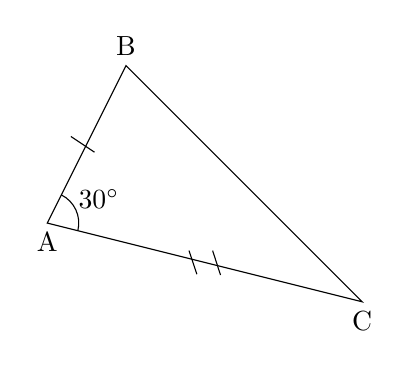
\begin{tikzpicture}
    \coordinate (A) at (0,0);
    \coordinate (B) at (1,2);
    \coordinate (C) at (4, -1);

    \draw   (A) node[below] {A} --
            (B) node[above] {B} --
            (C) node[below] {C} -- cycle;
    
    \pic [draw, angle radius=4mm, angle eccentricity=1.8, "$30^\circ$"] {angle = C--A--B};
    
    \draw (0.3, 1.1) -- (0.6, 0.9);
    \draw (1.9, -0.65) -- (1.8, -0.35);
    \draw  (2.2, -0.66) -- (2.1, -0.35);

\end{tikzpicture}
\hspace{1.8cm}
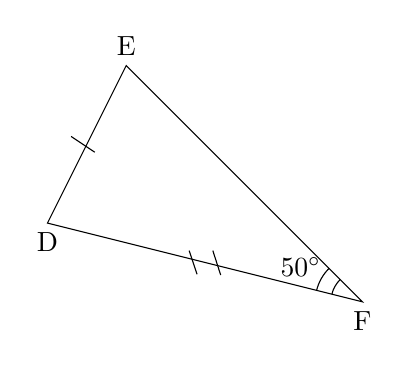
\begin{tikzpicture}
    \coordinate (D) at (0,0);
    \coordinate (E) at (1,2);
    \coordinate (F) at (4, -1);

    \draw   (D) node[below] {D} --
            (E) node[above] {E} --
            (F) node[below] {F} -- cycle;
    
    \pic [draw, angle radius=4mm, angle eccentricity=1, ""] {angle = E--F--D};
    \pic [draw, angle radius=6mm, angle eccentricity=1.5, "$50^\circ$"] {angle = E--F--D};
    
    \draw (0.3, 1.1) -- (0.6, 0.9);
    \draw (1.9, -0.65) -- (1.8, -0.35);
    \draw  (2.2, -0.66) -- (2.1, -0.35);

\end{tikzpicture}
\end{document}